% Рисуночки
\section{Конструкторская часть}
\subsection{Описания алгоритмов}

\hspace{1.25cm}
На основании теоретических измышлений были разработаны алгоритмы, вычисляющие произведение матриц тремя способами: стандартным, Винограда и оптимизированным Винограда. Блок-схемы этих алгоритмов приведены на рисунках \ref{fig:block_1_1} и \ref{fig:block_1_2} (стандартный), рисунках \ref{fig:block_2_1}, \ref{fig:block_2_2} и \ref{fig:block_2_3} (Винограда) и рисунках \ref{fig:block_3_1}, \ref{fig:block_3_2} и \ref{fig:block_3_3} (оптимизированный Винограда).

Вариант оптимизации: двоичный сдвиг вместо умножения на 2; объединение III и IV частей алгоритма Винограда; вынос начальной итерации из каждого внешнего цикла.

\begin{figure}[H]
    \centering
    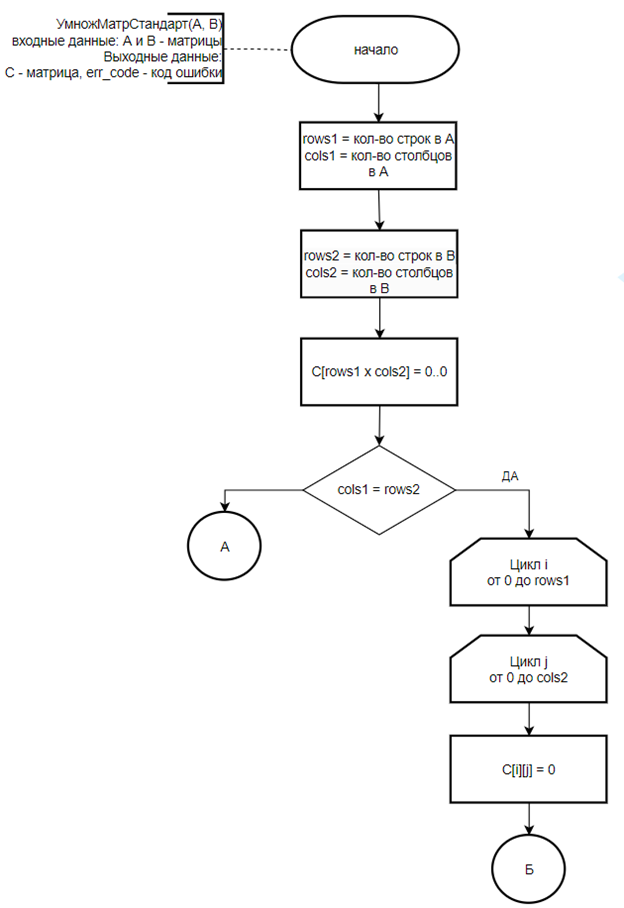
\includegraphics[width=0.9\textwidth]{img/block_1_1.png}
    \caption{Блок-схема стандартного алгоритма умножения матриц}
    \label{fig:block_1_1}
\end{figure}


\begin{figure}[H]
    \centering
    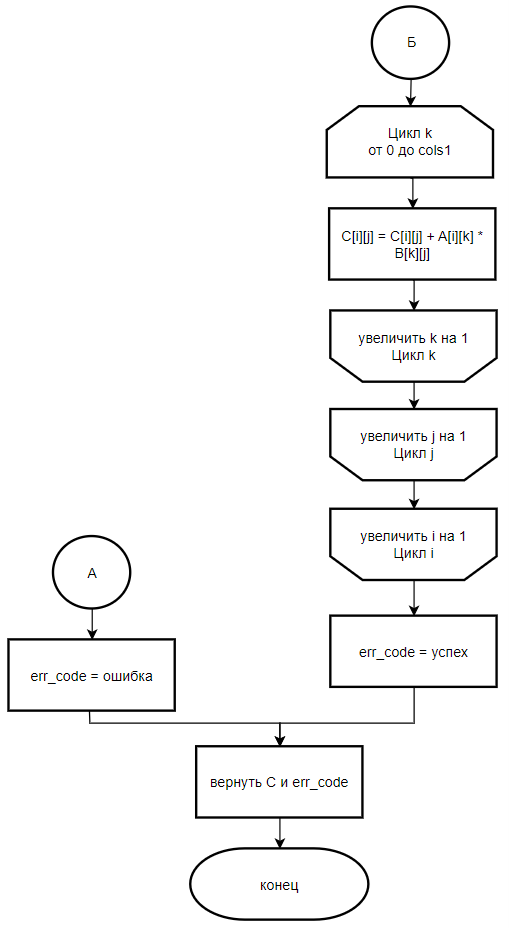
\includegraphics[width=0.8\textwidth]{img/block_1_2.png}
    \caption{Блок-схема стандартного алгоритма умножения матриц (продолжение)}
    \label{fig:block_1_2}
\end{figure}

\begin{figure}[H]
    \centering
    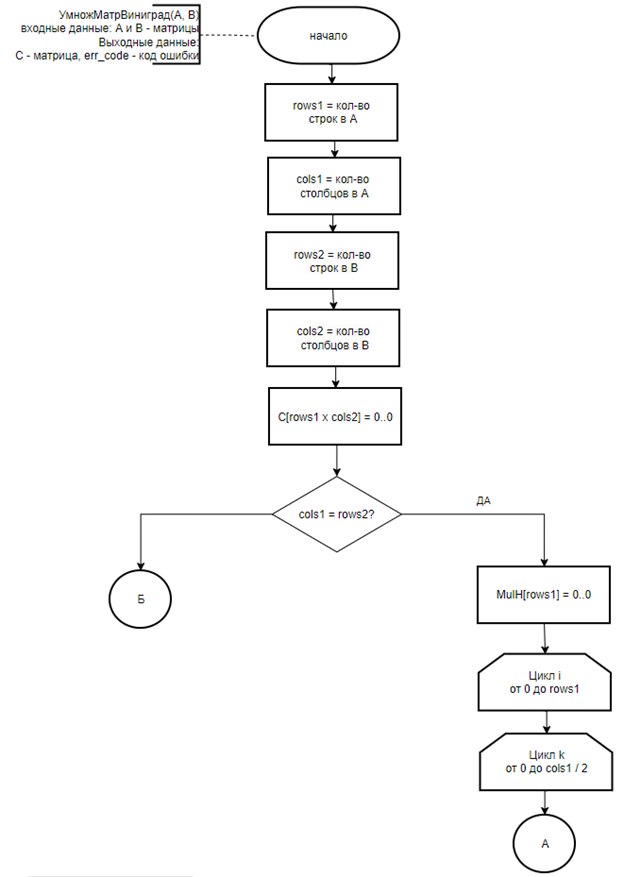
\includegraphics[width=1.05\textwidth]{img/block_2_1.png}
    \caption{Блок-схема алгоритма Винограда умножения матриц}
    \label{fig:block_2_1}
\end{figure}

\begin{figure}[H]
    \centering
    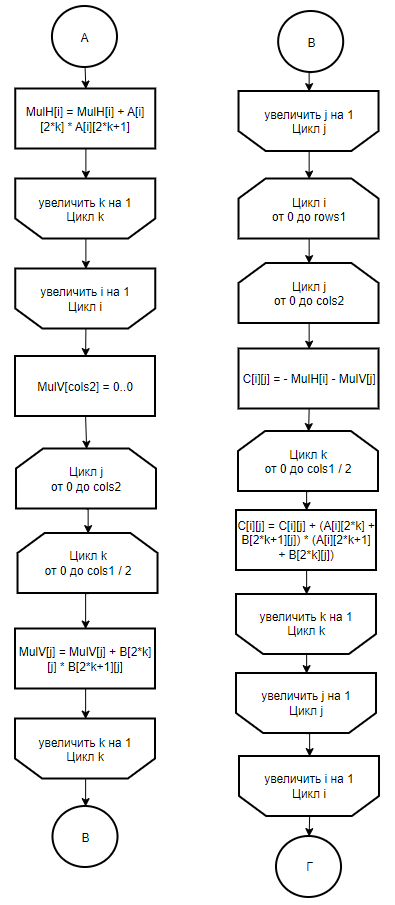
\includegraphics[width=0.65\textwidth]{img/block_2_2.png}
    \caption{Блок-схема алгоритма Винограда умножения матриц (продолжение)}
    \label{fig:block_2_2}
\end{figure}

\begin{figure}[H]
    \centering
    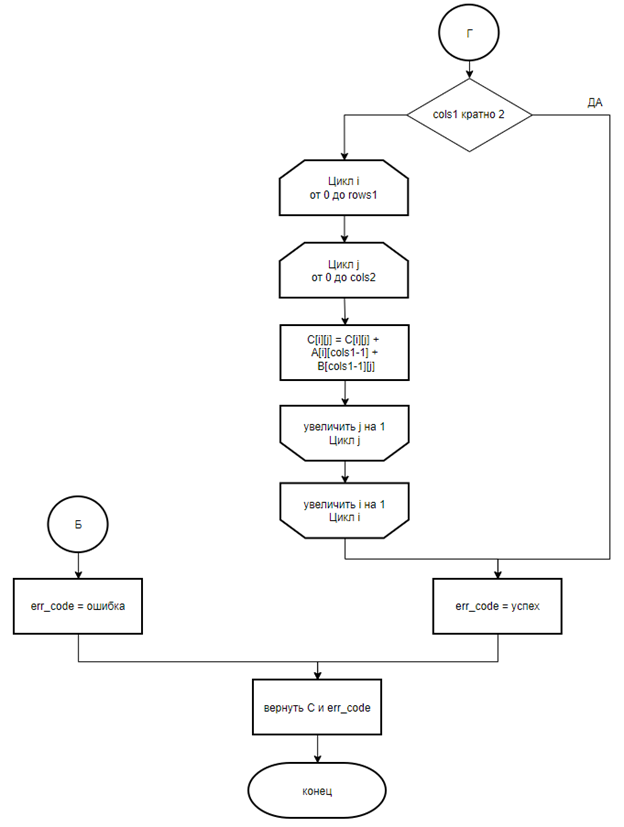
\includegraphics[width=1.02\textwidth]{img/block_2_3.png}
    \caption{Блок-схема алгоритма Винограда умножения матриц (продолжение 2)}
    \label{fig:block_2_3}
\end{figure}

\begin{figure}[H]
    \centering
    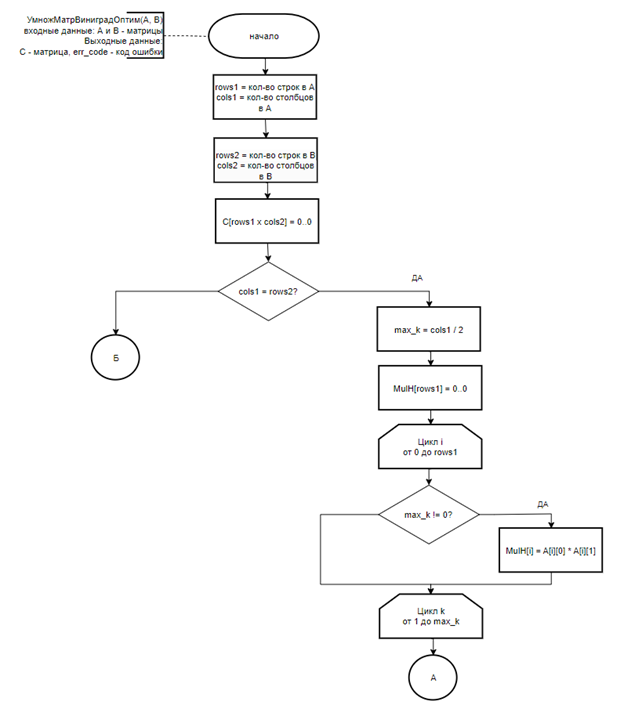
\includegraphics[width=1.05\textwidth]{img/block_3_1.png}
    \caption{Блок-схема оптимизированного алгоритма Винограда умножения матриц}
    \label{fig:block_3_1}
\end{figure}

\begin{figure}[H]
    \centering
    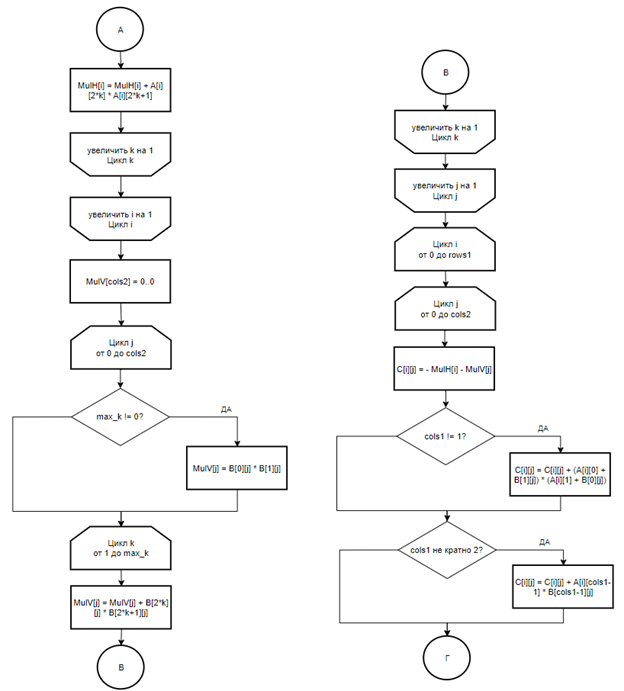
\includegraphics[width=1.05\textwidth]{img/block_3_2.png}
    \caption{Блок-схема оптимизированного алгоритма Винограда умножения матриц (продолжение)}
    \label{fig:block_3_2}
\end{figure}

\begin{figure}[H]
    \centering
    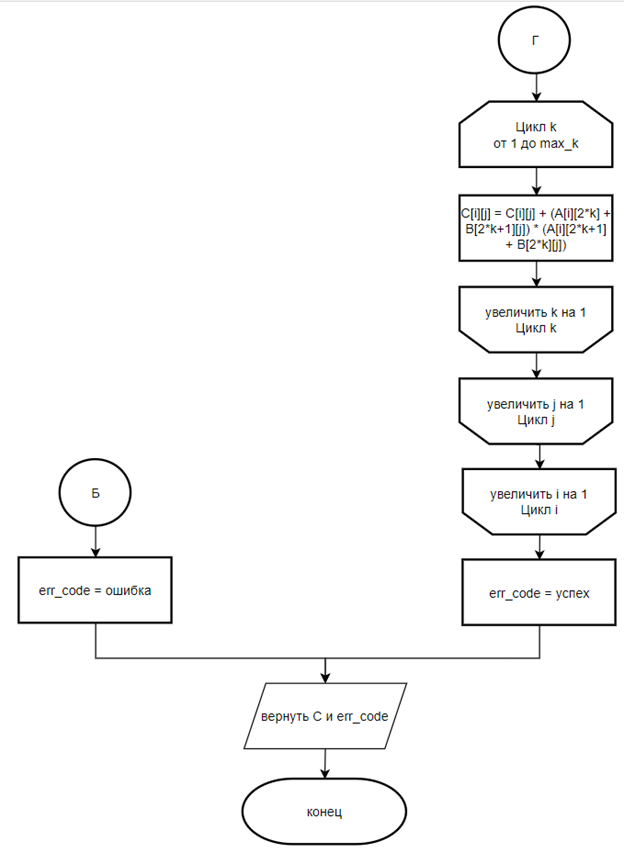
\includegraphics[width=1.02\textwidth]{img/block_3_3.png}
    \caption{Блок-схема оптимизированного алгоритма Винограда умножения матриц (продолжение 2)}
    \label{fig:block_3_3}
\end{figure}

\subsection{Модель вычислений}

\hspace{1.25cm}
Введём правила, по которым будем оценивать ресурсную эффективность:

\begin{enumerate}

\item трудоёмкость базовых операций

Примем единичной трудоёмкость следующих операций:

=, +, -, +=, -=, ==, !=, <, >, <=, >=, [], >>, <<, \&\&, ||, |=, \&=

Трудоёмкость примем за 2:

/, *, *=, /=, %

\item трудоёмкость оператора цикла

Пусть для цикла вида:

for (инициализация, сравнение, инкремент)\\
\{ тело \}

известны трудоёмкости соответствующих блоков:

\[f_{\text{иниц}}, f_{\text{срав}}, f_{\text{инкрем}}, f_{\text{тела}} \]

Тогда трудоёмкость цикла с "n" итерациями имеет следующий вид:

\begin{equation}
    f_{\text{цикла}} = f_{\text{иниц}} + f_{\text{срав}} + n * (f_{\text{тела}} + f_{\text{инкрем}} + f_{\text{срав}})
\end{equation}


\item трудоёмкость условного оператора

Пусть трудоёмкость условного перехода равна нулю, тогда для условного оператора вида:

if (условие)\\
\{ блок 1 \}\\
else \\
\{ блок 2 \}

известны трудоёмкости соответствующих блоков:

\[f_1, f_2, f_{\text{усл}}\]

Тогда трудоёмкость будет оценена как:

\begin{equation}
    f_{\text{if}} = f_{\text{усл}} + 
    \begin{cases}
      \text{min}(f_1, f_2) & \text{лучший случай}; \\
      \text{max}(f_1, f_2) & \text{худший случай}.
    \end{cases}
\end{equation}

Примечание: при $f_1 = f_2$ разделения на случаи не будет.

\end{enumerate}

\subsection{Расчёт трудоёмкости алгоритмов}

\hspace{1.25cm}
Далее будет рассчитана трудоёмкость стандартного алгоритма умножения матриц, Винограда и оптимизированного алгоритма Винограда.

Примечание: выделение памяти под матрицу не будет включено в расчёты трудоёмкости как не самая тяжёлая операция, присутствующая во всех алгоритмах.

\subsubsection{Стандартный алгоритм умножения матриц}

\hspace{1.25cm}
Трудоёмкость стандартного алгоритма умножения матриц состоит из пяти основных компонент:

\begin{enumerate}

\item внешний цикл по i в диапазоне [0, M)
\begin{equation}
f_i = 1 + M * (1 + 1 + f_{\text{тела}}) + 1
\end{equation}

\item внутренний цикл по j в диапазоне [0, Q)
\begin{equation}
f_i = 1 + Q * (1 + 1 + f_{\text{тела}}) + 1
\end{equation}

\item инициализация текущего элемента нулевым значением с трудоёмкостью равной 3


\item внутренний цикл по k в диапазоне [0, N)
\begin{equation}
f_i = 1 + N * (1 + 1 + f_{\text{тела}}) + 1
\end{equation}

\item добавление к текущему элементу произведения чисел из соответствующих строки и столбца с трудоёмкостью равной 12

\end{enumerate}

Подставив в одну формулу, получим итоговую трудоёмкость:
\begin{equation}
f_{\text{стандарт}} = 2 + M * (4 + Q * (4 + 3 + N * (2 + 12))) = 14 * MNQ + 7 * MQ + 4 * M  + 2
\end{equation}

\subsubsection{Алгоритм Винограда умножения матриц}

\hspace{1.25cm}
Трудоёмкость алгоритма Винограда умножения матриц состоит из четырёх основных компонент:

\begin{enumerate}

\item заполнение массива MulH
\begin{equation}
f_{MulH} = 2 + M * (2 + 4 + N/2 * (4 + 4 + 11)) = 19/2 * MN + 6 * M + 2
\end{equation}

\item заполнение массива MulV
\begin{equation}
f_{MulV} = 2 + Q * (2 + 4 + N/2 * (4 + 4 + 11)) = 19/2 * QN + 6 * Q + 2
\end{equation}

\item заполнение матрицы C
\begin{equation}
f_C = 2 + M * (2 + 2 + Q * (2 + 7 + 4 + N/2 * (4 + 6 + 22))) = 32/2 * MNQ + 13 * MQ + 4 * M + 2
\end{equation}


\item поправка на нечётность N
\begin{equation}
f_{odd_N} = 3 + 
    \begin{cases}
      0 & \text{л.c.(N чётно)}; \\
      2 + M * (2 + 2 + Q * (2 + 11)) & \text{х.c.(N нечётно)}.
    \end{cases}
= 3 +
	\begin{cases}
      0 & \text{л.с.} \\
      13 * MQ + NM + 2 & \text{х.c.}
    \end{cases}
\end{equation}

\end{enumerate}

Подставив в одну формулу, получим итоговую трудоёмкость:
\[f_{\text{Виноград}} = f_{MulH} + f_{MulV} + f_C + f_{odd_N}\]

\begin{multline}
f_{\text{Виноград}} = \frac{19}{2} MN + 6M + 2 + \frac{19}{2} QN + 6Q + 2 + \frac{32}{2} MNQ + 13MQ + 4M + 2 + 3 + \\
+ \begin{cases}
0 & \text{л.с.} \\
13MQ + NM + 2 & \text{х.c.}
\end{cases}
\end{multline}

\begin{equation}
\begin{aligned}
f_{\text{Виноград}} &= \frac{32}{2} MNQ + 13 MQ + \frac{19}{2} MN + \frac{19}{2} QN + 10 M + 6 Q + 9 + \\
&\quad + \begin{cases}
0 & \text{л.с.} \\
13 MQ + MN + 2 & \text{х.c.}
\end{cases}
\end{aligned}
\end{equation}

\subsubsection{Оптимизированный алгоритм Винограда умножения матриц}

\hspace{1.25cm}
Вариант оптимизации: двоичный сдвиг вместо умножения на 2; объединение III и IV частей алгоритма Винограда; вынос начальной итерации из каждого внешнего цикла.

Трудоёмкость оптимизированного алгоритма Винограда умножения матриц состоит из трёх основных компонент (в связи с оптимизацией --- объединением III и IV частей):

\begin{enumerate}

\item заполнение массива MulH
\[
f_{MulH} = 2 + M * (2 + 1 + 
	\begin{cases}
      0 & \text{л.c.(cols1 < 2)}; \\
      8 & \text{х.c.(cols1 >= 2)}.
    \end{cases}
     + 2 + (N/2 - 1) * (2 + 4 + 9))
\]

\begin{equation}
f_{MulH} = 2 - 10 * M + 15/2 * M * N + 
	\begin{cases}
      0 & \text{л.c.(cols1 < 2)}; \\
      8 * M & \text{х.c.(cols1 >= 2)}.
    \end{cases}
\end{equation}

\item заполнение массива MulV
\[
f_{MulV} = 2 + Q * (2 + 1 + 
	\begin{cases}
      0 & \text{л.c.(cols1 < 2)}; \\
      8 & \text{х.c.(cols1 >= 2)}.
    \end{cases}
     + 2 + (N/2 - 1) * (2 + 4 + 9))
\]

\begin{equation}
f_{MulV} = 2 - 10 * Q + 15/2 * Q * N + 
	\begin{cases}
      0 & \text{л.c.(cols1 < 2)}; \\
      8 * Q & \text{х.c.(cols1 >= 2)}.
    \end{cases}
\end{equation}

\item заполнение матрицы C
\begin{multline*}
f_C = 2 + M \cdot ( 2 + 2 + Q \cdot ( 2 + 7 + 1 + 
  \begin{cases}
    0 & \text{л.c.(cols1 != 1)}; \\
    18 & \text{х.c.(cols1 != 1)}.
  \end{cases}
+ 3 + 
  \begin{cases}
    0 & \text{л.c.(cols1 \vdots 2)}; \\
    14 & \text{х.c.(cols1 \vdots 2)}.
  \end{cases}  \\
+ 2 + \left( \frac{N}{2} - 1 \right) \cdot (2 + 24)))
\end{multline*}

\begin{multline}
f_C = 2 + 4 \cdot M - 11 \cdot M \cdot Q + 13 \cdot NMQ + 
	\begin{cases}
      0 & \text{л.c.(cols1 != 1)}; \\
      18 \cdot MQ & \text{х.c.(cols1 != 1)}.
    \end{cases} + \\ + 
    \begin{cases}
      0 & \text{л.c.(cols1 \vdots 2)}; \\
      14 \cdot MQ & \text{х.c.(cols1 \vdots 2)}.
    \end{cases}
\end{multline}

\end{enumerate}

Подставив в одну формулу, получим итоговую трудоёмкость:
\[f_{\text{Виноград}} = 2 + f_{MulH} + f_{MulV} + f_C\]

Примечание: 2 добавляется за счёт вычисления заранее cols1 / 2.

\begin{multline}
f_{\text{Виноград}} = 2 + 2 - 10 \cdot M + 15/2 \cdot MN + 
	\begin{cases}
      0 & \text{л.c.(cols1 < 2)}; \\
      8 \cdot M & \text{х.c.(cols1 >= 2)}.
    \end{cases}
 + 2 + Q \cdot (2 + 1 + \\ + 
	\begin{cases}
      0 & \text{л.c.(cols1 < 2)}; \\
      8 & \text{х.c.(cols1 >= 2)}.
    \end{cases}
 + 2 + (N/2 - 1) \cdot (2 + 4 + 9))
 + 2 + 4 \cdot M - 11 \cdot M \cdot Q + 13 \cdot NMQ + \\ +
	\begin{cases}
      0 & \text{л.c.(cols1 != 1)}; \\
      18 \cdot MQ & \text{х.c.(cols1 != 1)}.
    \end{cases} + 
    \begin{cases}
      0 & \text{л.c.(cols1 \vdots 2)}; \\
      14 \cdot MQ & \text{х.c.(cols1 \vdots 2)}.
    \end{cases}
\end{multline}

\subsection*{Вывод}

\hspace{1.25cm}
На основании теоретических измышлений были разработаны алгоритмы, вычисляющие произведение матриц тремя способами (стандартным, Винограда и оптимизированным Винограда), составлены блок-схемы этих алгоритмов. Была введена модель вычислений и рассчитаны трудоёмкости трёх алгоритмов умножения матриц.По полученным формулам можно сделать вывод, что алгоритм Винограда менее трудоёмок чем стандартный алгоритм умножения матриц, за счёт уменьшения числа умножений и вычисленных заранее значений, которые могут использоваться повторно. Благодаря оптимизациям по варианту третий алгоритм выгоднее по вычислительной сложности, чем алгоритм Винограда.

\newpage